In this section we will reason about the \emph{correctness of the implementation}.

We will be relying on the unit and integration test suite that has been created along with the algorithm.
It should be noted, that unit tests alone will not give a \emph{mathematical} proof of correctness, or total correctness (the former proves input-output correctness, while the latter also includes proof of termination). However, with a well-tested codebase we can almost certainly tell with a \emph{high degree of confidence}, that the code performs according to the specifications.

\subsection{Generalizer tests}

For each built-in generalizer implementation a corresponding test suite verifies the correct behavior. Without getting too much into the details, Figure~\ref{fig:generalizer_tests} shows a summary of the tests and their locations.

\vspace{\baselineskip}
\begin{figure}[H]
    \centering
    \small
    \begin{tabular}{r p{8cm}}
        \toprule
        \textbf{File} & \textbf{Functionality} \\
        \midrule
        \texttt{suppressor\_test.go}               & verifies basic suppression functionality \\
        \texttt{hierarchy\_test.go}                & basic \& auto builder, including edge cases for non-full trees and invalid input \\
        \texttt{hierarchy\_generalizer\_test.go}   & generalization to different levels, and related edge cases, benchmarks \\
        \texttt{range\_generalizer\_test.go}       & tests for int \& float ranges, including range validation, virtual hierarchy splitting and levels \\
        \texttt{prefix\_generalizer\_test.go}      & tests the prefix generalization logic, including validation of input \\
        \bottomrule
    \end{tabular}
    \caption{Generalizer Tests}\label{fig:generalizer_tests}
\end{figure}

\subsection{Core algorithm tests}

\subsubsection{Cost graph tests}
These tests cover the building and edge-cost calculation of cost graphs. The test suite in \texttt{cost\_test.go} deals with verifying the cost calculation formula. Another test suite verifies that the  cost-graph is built properly. In these tests the input is always a \emph{table}, and we verify, that the structure and edge-costs of the output graph is as expected. Tests also cover edge cases, like invalid data in the table, invalid generalizer for the column and empty input. The cost graph test suite is located in \texttt{cost\_graph\_test.go}.

\subsubsection{Forest building tests}
The tests for the forest building algorithm are located in \texttt{anon\_graph\_test.go}, and they verify the following aspects of the algorithm:
\begin{itemize}
    \setstretch{1.0}
    \item a correct component should be picked for extension
    \item a correct vertex should be picked as source vertex
    \item a correct vertex should be picked as target vertex
    \item forest (tree) properties are not violated after the new edge is added
\end{itemize}

\subsubsection{Decompose tests}
The decompose step is a rather complex step in the core algorithm. The test suite in the file \texttt{decompose\_test.go} tries to deal with this complexity. With the proper set of helper methods however, the tests in it are still readable and relatively easy to follow. An example can be seen on Figure~\ref{lst:decompose_test}.

Tests in the decompose suite are centered around the verification of the following:
\begin{itemize}
    \setstretch{1.0}
    \item oversized threshold calculation logic
    \item component picked for decomposition is actually oversized
    \item cut types A through D (see Section~\ref{subsec:algorithm-to-decompose-oversized-components})
    \item handling of Steiner's vertices
    \item the algorithm stops when there are no more oversized components in the forest
\end{itemize}

\begin{lstlisting}[caption=A test for Decompose Cut type B,label=lst:decompose_test,float,floatplacement=H]
//            ------- 0 ------
//           |                |
//      ---- 1 ----           6
//     |     |     |          |
//     2     3     4          7
//           |
//           5
//
//  u := 0, v := 1, k := 4, s > 2k-1
//  s-t == k-1
func TestPartition_TypeBCut(t *testing.T) {
    g := GetUndirectedTestGraph2()
    d := NewDecomposer(g, 4)
    u := g.Node(0)
    v := g.Node(1)
    d.performCutTypeB(u, v)
    testutil.AssertVertexReplaced(t, g, 1, 8, 2, 3, 4)
}
\end{lstlisting}

\subsubsection{Anonoymizer tests}
Last, but not least the tests in \texttt{anonymize\_test.go} check, that all the above work well together. They call the \texttt{Anonymizer} for a set of test input tables, and verify that \emph{k-anonymity} on the output is not violated. This is done by ensuring, that in the resulting output for any given row at least \(k-1\) other rows must be the same partition. (See Listing~\ref{lst:test_k_anonymity}.)

\subsection{Insufficiency of identifier truncation}\label{subsec:insuff}

Before diving into the definition of k-anonymity, let's take the previous example a little bit further, and consider the following patient data taken from the hospital's database:

\begin{figure}[H]
    \centering
    \begin{tabular}{c l c l l c l}
        \toprule
        \textbf{SSN} & \textbf{Name} & \textbf{Age} & \textbf{Race} & \textbf{Gender} & \textbf{Zip Code} & \textbf{Disease} \\
        \midrule
        1001 & John Smith  & 34 & White & Male   & 18500 & Flu \\
        1002 & Eva Brown   & 27 & Asian & Female & 18200 & Cancer \\
        1003 & Anne Parker & 17 & White & Female & 18500 & Hypertension \\
        1004 & Mark Wayne  & 34 & Black & Male   & 18200 & Flu \\
        \bottomrule
    \end{tabular}
    \caption{Example patient data}\label{fig:example-patient-data}
\end{figure}

In order to attempt to remove personal information from the data, one --- albeit naïve --- approach the hospital could choose is to simply \textit{truncate} all fields that contain identifiers.
In the above example they will be the \textit{social security number} and \textit{name} fields.
The resulting table will look something like this:

\begin{figure}[H]
    \centering
    \begin{tabular}{c l l c l}
        \toprule
        \textbf{Age} & \textbf{Race} & \textbf{Gender} & \textbf{Zip Code} & \textbf{Disease} \\
        \midrule
        34 & White & Male   & 18500 & Flu \\
        27 & Asian & Female & 18200 & Cancer \\
        17 & White & Female & 18500 & Hypertension \\
        34 & Black & Male   & 18200 & Flu \\
        \bottomrule
    \end{tabular}
    \caption{Truncated patient data}\label{fig:truncated-patient-data}
\end{figure}

Unfortunately by using an external public database --- for example census records or a phone book --- an attacker could still piece together which person was diagnosed with which disease, thus rendering the hospital's data protection method useless.
This is called a \textbf{\textit{table join attack}}:

\begin{figure}[H]
    \centering
    \begin{tabular}{c l c}
        \toprule
        \textbf{Age} & \textbf{Name} & \textbf{Zip Code} \\
        \midrule
        34 & John Smith  & 18500 \\
        27 & Eva Brown   & 18200 \\
        17 & Anne Parker & 18500 \\
        34 & Mark Wayne  & 18200 \\
        \bottomrule
    \end{tabular}
    \caption{Census data}\label{fig:census-data}
\end{figure}

\begin{figure}[H]
    \centering
    \begin{tabular}{l c l l c l}
        \toprule
        \textbf{Name} & \color{red}{\textbf{Age}} & \textbf{Race} & \textbf{Gender} & \color{red}{\textbf{Zip Code}} & \textbf{Disease} \\
        \midrule
        John Smith  & \color{red}{34} & White & Male   & \color{red}{18500} & Flu \\
        Eva Brown   & \color{red}{27} & Asian & Female & \color{red}{18200} & Cancer \\
        Anne Parker & \color{red}{17} & White & Female & \color{red}{18500} & Hypertension \\
        Mark Wayne  & \color{red}{34} & Black & Male   & \color{red}{18200} & Flu \\
        \bottomrule
    \end{tabular}
    \caption{Patient data restored with join attack}\label{fig:joined-patient-data}
\end{figure}


One might think, that this does not usually happen outside of fabricated examples.
Unfortunately, as Sweeney observed~\cite{sweeney} for 87\% of the U.S.\ population the combination of date of birth, gender and zip code corresponded to a unique person~\cite{aggarwal} --- which could easily make the above example reality.

\subsection{Data model}\label{subsec:data_model}

Most anonymization algorithms work on data tables with a concrete \textit{schema} so we will adopt this model as well.
Tables can also be viewed as \textit{n} row vectors, or \textit{tuples}.
Each tuple represents an individual piece of data, and consists of \textit{m} attributes \((c_1, c_2, \ldots, c_m)\).
Attributes are sometimes also referred to as \textit{dimensions}.

\subsubsection{Attribute types}

\paragraph{identifiers:} these attributes by themselves alone can be used to identify the person whom the data belongs to without the need to reference any other attributes.
It is easy to see, that anonymization algorithms will always need to truncate or suppress all of these attributes from the final anonymized data set.

\paragraph{quasi-identifiers:} as illustrated by the examples in Section~\ref{subsec:insuff} some attributes are not identifiers themselves but can still be used in conjunction with external data sources to identify the concrete person.
These attributes are \textit{quasi-identifier} attributes, and will be subject to some level of generalization or suppression based on the algorithm being used (refer to the next section called \textit{`Data hiding techniques`} for a more precise explanation of generalization and suppression).

\paragraph{non-identifiers:} attributes, which the \textit{data controller} deems irrelevant in the context of anonymization are non-identifiers.
We can often extract useful statistics from their values, but they are meaningless without pairing them with additional attributes.

\subsubsection{Data hiding techniques} In order to remove sensitive data from a database, anonymization algorithms use common data hiding techniques.
In this section we will briefly introduce two commonly used, and illustrate how they work on simple examples.

\paragraph{suppression} is very similar to truncating all sensitive data values.
When looking at a single attribute (like age) in a database, truncating it would redact \textit{all} values.
Suppression on the other hand redacts \textit{some} of the values, while retaining the rest~\cite{aggarwal}.
Which values are suppressed and which values are retained is decided by the anonymization algorithm, which considers several different factors.

Figure~\ref{fig:suppression_example} shows the anonymization of a table using suppression only, along the quasi-identifiers Name, Age and Gender:

\begin{figure}[H]
    \centering
    \begin{tabular}{l c l c}
        \toprule
        \textbf{Name} & \textbf{Age} & \textbf{Gender} & \textbf{Salary} \\
        \midrule
        John & 25 & Male   & 50000 \\
        Mark & 30 & Male   & 65000 \\
        Jill & 24 & Female & 45000 \\
        Jane & 24 & Female & 70000 \\
        \bottomrule
    \end{tabular}
    \quad
    \begin{tabular}{l c l c}
        \toprule
        \textbf{Name} & \textbf{Age} & \textbf{Gender} & \textbf{Salary} \\
        \midrule
        * & *  & Male   & 50000 \\
        * & *  & Male   & 65000 \\
        * & 24 & Female & 45000 \\
        * & 24 & Female & 70000 \\
        \bottomrule
    \end{tabular}
    \caption{Suppression}\label{fig:suppression_example}
\end{figure}

\paragraph{generalization} replaces values with less specific, but semantically consistent values from the same domain.
For example a date can be made more generic by omitting the days and even more so by reducing it to the year only. (Note, that suppression is basically a special case of generalization --- we can create a special generalization function, which maps every value to a suppressed value in one step.)

Figure~\ref{fig:generalization} shows the anonymization of a table using generalization along the quasi-identifiers Name, Age and Gender:

Generalization is a core concept when talking about the \textit{k-anonymity with generalization} problem.
The algorithm described in Chapter~\ref{ch:chapter_algorithm} uses generalization at its core: both to determine which rows to put into the same partition, and during the final step when the original rows are anonymized.

\subsection{Generalization API requirements}\label{subsec:generalization_requirements}
The library needs to provide a way for the API user to define how to generalize certain data types in their schema.
The implementation also needs to be flexible, but convenient and easy-to-use at the same time.
We want to make sure, that the implementation can satisfy at least the following requirements:

\begin{itemize}
    \setstretch{1.0}
    \item supports \textbf{generalization hierarchy}, with convenient declaration
    \item supports \textbf{suppression}
    \item supports \textbf{sets, ranges}
    \item supports \textbf{text}
    \item supports \textbf{non}-hierarchy based generalization
    \item custom generalizers can be created by \textbf{implementing an interface}
\end{itemize}

Until now we have only discussed \textit{hierarchy}-based generalization, and for the theoretical discussion of the anonymization algorithm it was perfectly sufficient.
You can create a generalization hierarchy for basically any data type --- even though the number of levels and the number of partitions on a given level may end up very large, or even infinite.

It is important to note however, that in real-life scenarios this is not always feasible.
Storage, operating memory and computing time is finite, which means that for some dimensions (like \textit{text}) we will need to apply a different type of abstraction.

\subsection{Generalization implementation}\label{subsec:generalization-implementation}
Based on the requirements outlined in~\ref{subsec:generalization_requirements} we can define the interface of a \texttt{Generalizer}.
Note, that since Go is not a classic object oriented language, a traditional class-hierarchy is not present in the design.
What we do have in our toolkit are \textit{interfaces} and \textit{composition}.

We define the \texttt{Generalizer} interface with the following operations (refer to Figure~\ref{fig:generalization_package}):
\begin{enumerate}
    \setstretch{1.0}
    \item generalize a partition \textit{n} times
    \item get the maximum number of levels of generalization
\end{enumerate}
Remember, that a partition can either contain a single value, or a set of values, so it makes sense that the \texttt{Generalize} method takes and returns a \texttt{Partition}.
It is also essential to know the maximum levels of generalization in advance, otherwise we wouldn't be able to compute the scaled generalization cost when comparing two partitions.
There is a third convenience method on the interface which defines how to create a \texttt{Partition} from a raw value.
The actual implementation of this may vary in each type that implements the interface.

\vspace{\baselineskip}
\input{chapter03/figures/generalization-package.tex}


\subsection{Suppressor}
\begin{lstlisting}[caption=Suppresor implementation,label=lst:suppressor,float,floatplacement=H]
type Suppressor struct {
}

func (s *Suppressor) Generalize(p partition.Partition, n int) partition.Partition {
    if n == 0 {
        return p
    }
    if n == 1 {
        return s.InitItem("*")
    }
    return nil
}

func (s *Suppressor) Levels() int {
    return 2
}

func (s *Suppressor) InitItem(item interface{}) partition.Partition {
    return partition.NewItem(item)
}
\end{lstlisting}

\subsection{HierarchyGeneralizer}\label{subsec:hierarchy_generalizer}
\texttt{HierarchyGeneralizer} represents generalization hierarchies in the classic sense that has been outlined in~\ref{subsec:data_model}.
This generalizer will \textit{contain} an actual \texttt{Hierarchy} --- as seen on Figure~\ref{fig:generalization_package}.
The \texttt{Hierarchy} interface has functions to navigate the partitions within the hierarchy based on the parent-child relationships, a function to return the number of levels within the hierarchy and additional helper functions.
The \texttt{hierarchy} package also contains helper functions to make it easy for the end-user to build it from a set of items.

\paragraph{Manual hierarchy:} We will now show how to manually declare a simple grade hierarchy similar to the one introduced on Figure~\ref{fig:grades-hierarchy}, albeit with a lesser number of grades for simplicity's sake. The full code listing can be seen on Listing~\ref{lst:grade_hierarchy}.

\input{chapter03/listings/grade-hierarchy.tex}

In order to build the hierarchy, we need to describe it from top to bottom.
Recall, that the top level of the hierarchy contains a single partition with every item in the domain.
We then add the children of this partition as new sets, continuing until we reach the lowest level, where each partition contains only a single item.

\paragraph{Automatic hierarchy:} another, more convenient way to build a hierarchy is by using the included \texttt{AutoBuild} function. It takes two parameters: the amount of children a node should have, and a variadic array of the items to partition. The function will build a valid hierarchy on-the-fly by splitting the set of items to the specified child partitions on each level, until only singleton partitions remain. (Note, that we may still get an error in case there is a problem with the arguments, for example when the desired child count is larger than the available items.) The builder may create partitions with less than the specified amount of children in cases when there aren't enough items. This often happens when the original number of items is not divisible by the desired child count.

 We now show how to build the same grade hierarchy automatically. Listing~\ref{lst:auto_build} demonstrates how to specify the child count and the items. By passing in \textit{3} as the desired child count we achieve the exact same result as the previous example.

\input{chapter03/listings/grade-hierarchy-auto.tex}

\paragraph{Validation} A hierarchy will also be \textit{validated} when it is built.
Validation will enforce, that:
\begin{itemize}
    \setstretch{1.0}
    \item an item can only appear once on a given level
    \item the superset of partitions on each level contains all items from the domain
\end{itemize}

\subsection{RangeGeneralizer}
\vspace{\baselineskip}
\input{chapter03/figures/partition-hierarchy.tex}

We have previously seen how partitions are the building blocks of generalization.
They are very similar to \textit{sets} in the mathematical sense.
In a standard generalization hierarchy we only needed to use \texttt{Partition}, \texttt{Item} and \texttt{Set}. (See Figure~\ref{fig:partition_hierarchy}.)

Representing larger ranges of numbers with the above strategy however would be very tedious.
We would not only have to write up each number on every level of the hierarchy, but also need to determine at what number the ranges are split up into partitions, and assign the proper parent-child relationships.
It is too much work, and in case of floating point numbers not even possible.
One option could be to generate a hierarchy with a \texttt{HierarchBuilder} as mentioned in~\ref{subsec:hierarchy_generalizer}. This removes the manual work of building up the partitions, but still has the need to store the whole hierarchy in the memory. For very large sets this could be inefficient.
We need a more feasible way of describing these types of dimensions.
This is why the \texttt{RangeGeneralizer} has been built into the library.

As it can be seen from Figure~\ref{fig:partition_hierarchy}, a \texttt{Range} interface can be derived from \texttt{Partition} which will deal with representing and splitting the ranges.
Its two implementations are \texttt{IntRange} and \texttt{FloatRange}.

The basic idea is, that after a number range is declared with its minimum and maximum boundaries, we can dynamically compute the partitions at the required level \emph{on the fly}.
Instead of keeping the full hierarchy in the memory, the \texttt{RangeGeneralizer} will \texttt{Split ()} the initial range the requested \texttt{n} number of times to arrive at the necessary generalization level.

\vspace{\baselineskip}
\input{chapter03/figures/range-generalizer.tex}

Figure~\ref{fig:range_generalizer} shows an example of this in action. (Nodes with gray dotted border represent only a visual aid for the reader, the algorithm does not need to compute them.) Let's assume we are generalizing a range of integers \([0\dots10]\).
If we are interested in what partition the value \(n=4\) would be generalized into on level \(l=1\), we need to split the range \(s=l_{\max}-l-1=3\) times.
After each step we need to keep splitting the partition in which the requested element exists.
After the required number of splits we arrive at the result (partition \([3\dots4]\)) without having to worry about constructing the actual generalization hierarchy at any point.
Note, that the distribution of the items in the partitions is actually handled by how the \texttt{Split ()} function is implemented for the corresponding \texttt{Range}.
In this case (and in the library) we are using a uniform distribution by splitting each range at the median value.

With some modification this strategy can implemented for floating point ranges as well, but the code will need to take floating point precision into account, and compare with a delta.


\subsection{PrefixGeneralizer}\label{subsec:prefix_generalizer}
The \texttt{PrefixGeneralizer} is another built-in generalizer, that does not rely on a fixed hierarchy. It deals with generalizing plain text data. As the name suggests, it will try to use different sized prefixes to see if two different strings can be collapsed into the same partition.

The input text will be interpreted as a series of words. The generalizer has a \texttt{MaxWords} setting, and it cannot handle text that has a larger word count. Note, that the actual length of words in characters is \textit{irrelevant} for this generalizer, and is only bounded by operative memory.

\paragraph{Example:} the example on Figure~\ref{fig:prefix_generalizer_1} shows how the prefix generalizer transforms two different sentences when different levels of generalization \textit{l} are selected. We assume, that \(MaxWords = 5\) for this example.

The first sentence only contains 3 words, so the \texttt{PrefixGeneralizer} will pad the last two slots. This makes it easy to compare the two sentences word-by-word. On levels 0, 1 and 2 the string prefixes are not equal. On level 3 the two strings are equal. Calculating the generalization cost for the two values would also be pretty simple: we divide the lowest level of generalization which assigns the two items into the same partition by the maximum levels of generalization: \(h/l_{\max} = 3/5\).

\vspace{\baselineskip}
\input{chapter03/figures/prefix-generalizer-1.tex}

Figure~\ref{fig:prefix_generalizer_2} illustrates what happens when the two strings differ in all prefixes. In this case the cost of generalization will be \(h/l_{\max} = 1 \), and both of the two strings are \textit{suppressed} (replaced with the ``*'' token).

\vspace{\baselineskip}
\input{chapter03/figures/prefix-generalizer-2.tex}

\subsection{Custom Generalizers}
Finally, if none of the built-in generalization techniques are adequate for a certain use case, the user of the library can still implement the \texttt{Generalizer} interface to provide a custom logic.

Recall from Section~\ref{sec:generalization}, that in order to properly implement the \texttt{Generalizer} interface, one has to implement the following methods:

\underline{\texttt{Levels () int}}: \\
This method should return the maximum number of times the generalizer can generalize the values. In hierarchy based generalizers it is usually the number of levels in the tree. It is important to note, that the levels are zero-indexed, which needs to be taken account when calculating the number of levels with a non-hierarchy based logic.

\underline{\texttt{Generalize (Partition, int) Partition}}: \\
This method should generalize the input partition n times (providing that \(n \le Levels ()\)) and return the resulting partition. The result will be used by the core anonymization algorithm when calculating the cost graph.

\underline{\texttt{InitItem (interface\{ \}) Partition}}: \\
Implement this method to tell how to initialize a raw value. In most cases you just want to wrap it into an \texttt{Item} or \texttt{Set}.

In most cases we can assume, that for each attribute a \textit{\textbf{generalization hierarchy}} exists~\cite{aggarwal}.
Each level of the generalization hierarchy corresponds to a partition of the attribute domain, and a refinement over the partitions on the previous level~\cite{samarati-sweeney}.
On the two opposing ends of the hierarchy we have singleton sets corresponding to the lack of generalization, and a single set containing all values from the domain corresponding to the highest level of generalization.

\begin{figure}[H]
    \centering
    \tikzset{every picture/.style={line width=0.75pt}} %set default line width to 0.75pt
    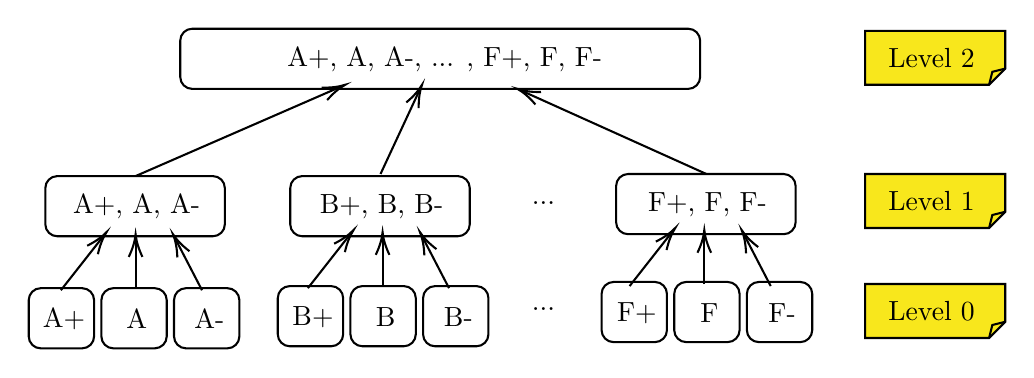
\begin{tikzpicture}[x=0.75pt,y=0.75pt,yscale=-1,xscale=1]
        %uncomment if require: \path (0,457); %set diagram left start at 0, and has height of 457

        %Rounded Rect [id:dp05055633926904224]
        \draw   (40,265.8) .. controls (40,262.6) and (42.6,260) .. (45.8,260) -- (120.7,260) .. controls (123.9,260) and (126.5,262.6) .. (126.5,265.8) -- (126.5,283.2) .. controls (126.5,286.4) and (123.9,289) .. (120.7,289) -- (45.8,289) .. controls (42.6,289) and (40,286.4) .. (40,283.2) -- cycle ;

        %Rounded Rect [id:dp15417219044870833]
        \draw   (158,265.8) .. controls (158,262.6) and (160.6,260) .. (163.8,260) -- (238.7,260) .. controls (241.9,260) and (244.5,262.6) .. (244.5,265.8) -- (244.5,283.2) .. controls (244.5,286.4) and (241.9,289) .. (238.7,289) -- (163.8,289) .. controls (160.6,289) and (158,286.4) .. (158,283.2) -- cycle ;

        %Rounded Rect [id:dp5566983339728413]
        \draw   (315,264.8) .. controls (315,261.6) and (317.6,259) .. (320.8,259) -- (395.7,259) .. controls (398.9,259) and (401.5,261.6) .. (401.5,264.8) -- (401.5,282.2) .. controls (401.5,285.4) and (398.9,288) .. (395.7,288) -- (320.8,288) .. controls (317.6,288) and (315,285.4) .. (315,282.2) -- cycle ;

        %Rounded Rect [id:dp14128108650523874]
        \draw   (32,319.8) .. controls (32,316.6) and (34.6,314) .. (37.8,314) -- (57.7,314) .. controls (60.9,314) and (63.5,316.6) .. (63.5,319.8) -- (63.5,337.2) .. controls (63.5,340.4) and (60.9,343) .. (57.7,343) -- (37.8,343) .. controls (34.6,343) and (32,340.4) .. (32,337.2) -- cycle ;

        %Rounded Rect [id:dp6850532710750563]
        \draw   (67,319.8) .. controls (67,316.6) and (69.6,314) .. (72.8,314) -- (92.7,314) .. controls (95.9,314) and (98.5,316.6) .. (98.5,319.8) -- (98.5,337.2) .. controls (98.5,340.4) and (95.9,343) .. (92.7,343) -- (72.8,343) .. controls (69.6,343) and (67,340.4) .. (67,337.2) -- cycle ;
        %Rounded Rect [id:dp49831794890726244]
        \draw   (102,319.8) .. controls (102,316.6) and (104.6,314) .. (107.8,314) -- (127.7,314) .. controls (130.9,314) and (133.5,316.6) .. (133.5,319.8) -- (133.5,337.2) .. controls (133.5,340.4) and (130.9,343) .. (127.7,343) -- (107.8,343) .. controls (104.6,343) and (102,340.4) .. (102,337.2) -- cycle ;
        %Rounded Rect [id:dp5034621708150937]
        \draw   (152,318.8) .. controls (152,315.6) and (154.6,313) .. (157.8,313) -- (177.7,313) .. controls (180.9,313) and (183.5,315.6) .. (183.5,318.8) -- (183.5,336.2) .. controls (183.5,339.4) and (180.9,342) .. (177.7,342) -- (157.8,342) .. controls (154.6,342) and (152,339.4) .. (152,336.2) -- cycle ;
        %Rounded Rect [id:dp4304422122223639]
        \draw   (187,318.8) .. controls (187,315.6) and (189.6,313) .. (192.8,313) -- (212.7,313) .. controls (215.9,313) and (218.5,315.6) .. (218.5,318.8) -- (218.5,336.2) .. controls (218.5,339.4) and (215.9,342) .. (212.7,342) -- (192.8,342) .. controls (189.6,342) and (187,339.4) .. (187,336.2) -- cycle ;
        %Rounded Rect [id:dp8079993361963536]
        \draw   (222,318.8) .. controls (222,315.6) and (224.6,313) .. (227.8,313) -- (247.7,313) .. controls (250.9,313) and (253.5,315.6) .. (253.5,318.8) -- (253.5,336.2) .. controls (253.5,339.4) and (250.9,342) .. (247.7,342) -- (227.8,342) .. controls (224.6,342) and (222,339.4) .. (222,336.2) -- cycle ;
        %Rounded Rect [id:dp3763444142614236]
        \draw   (308,316.8) .. controls (308,313.6) and (310.6,311) .. (313.8,311) -- (333.7,311) .. controls (336.9,311) and (339.5,313.6) .. (339.5,316.8) -- (339.5,334.2) .. controls (339.5,337.4) and (336.9,340) .. (333.7,340) -- (313.8,340) .. controls (310.6,340) and (308,337.4) .. (308,334.2) -- cycle ;
        %Rounded Rect [id:dp025410635634430356]
        \draw   (343,316.8) .. controls (343,313.6) and (345.6,311) .. (348.8,311) -- (368.7,311) .. controls (371.9,311) and (374.5,313.6) .. (374.5,316.8) -- (374.5,334.2) .. controls (374.5,337.4) and (371.9,340) .. (368.7,340) -- (348.8,340) .. controls (345.6,340) and (343,337.4) .. (343,334.2) -- cycle ;
        %Rounded Rect [id:dp6345478019954871]
        \draw   (378,316.8) .. controls (378,313.6) and (380.6,311) .. (383.8,311) -- (403.7,311) .. controls (406.9,311) and (409.5,313.6) .. (409.5,316.8) -- (409.5,334.2) .. controls (409.5,337.4) and (406.9,340) .. (403.7,340) -- (383.8,340) .. controls (380.6,340) and (378,337.4) .. (378,334.2) -- cycle ;
        %Rounded Rect [id:dp5704093284694525]
        \draw   (105,194.8) .. controls (105,191.6) and (107.6,189) .. (110.8,189) -- (349.7,189) .. controls (352.9,189) and (355.5,191.6) .. (355.5,194.8) -- (355.5,212.2) .. controls (355.5,215.4) and (352.9,218) .. (349.7,218) -- (110.8,218) .. controls (107.6,218) and (105,215.4) .. (105,212.2) -- cycle ;
        %Straight Lines [id:da5982931753916951]
        \draw    (47.5,315) -- (68.26,288.57) ;
        \draw [shift={(69.5,287)}, rotate = 488.16] [color={rgb, 255:red, 0; green, 0; blue, 0 }  ][line width=0.75]    (10.93,-3.29) .. controls (6.95,-1.4) and (3.31,-0.3) .. (0,0) .. controls (3.31,0.3) and (6.95,1.4) .. (10.93,3.29)   ;

        %Straight Lines [id:da7014066905322178]
        \draw    (83.5,314) -- (83.5,290) ;
        \draw [shift={(83.5,288)}, rotate = 450] [color={rgb, 255:red, 0; green, 0; blue, 0 }  ][line width=0.75]    (10.93,-3.29) .. controls (6.95,-1.4) and (3.31,-0.3) .. (0,0) .. controls (3.31,0.3) and (6.95,1.4) .. (10.93,3.29)   ;

        %Straight Lines [id:da7237438732675705]
        \draw    (115.5,315) -- (102.42,289.78) ;
        \draw [shift={(101.5,288)}, rotate = 422.59000000000003] [color={rgb, 255:red, 0; green, 0; blue, 0 }  ][line width=0.75]    (10.93,-3.29) .. controls (6.95,-1.4) and (3.31,-0.3) .. (0,0) .. controls (3.31,0.3) and (6.95,1.4) .. (10.93,3.29)   ;

        %Straight Lines [id:da9667373614001253]
        \draw    (166.5,314) -- (187.26,287.57) ;
        \draw [shift={(188.5,286)}, rotate = 488.16] [color={rgb, 255:red, 0; green, 0; blue, 0 }  ][line width=0.75]    (10.93,-3.29) .. controls (6.95,-1.4) and (3.31,-0.3) .. (0,0) .. controls (3.31,0.3) and (6.95,1.4) .. (10.93,3.29)   ;

        %Straight Lines [id:da4011582897955388]
        \draw    (202.5,313) -- (202.5,289) ;
        \draw [shift={(202.5,287)}, rotate = 450] [color={rgb, 255:red, 0; green, 0; blue, 0 }  ][line width=0.75]    (10.93,-3.29) .. controls (6.95,-1.4) and (3.31,-0.3) .. (0,0) .. controls (3.31,0.3) and (6.95,1.4) .. (10.93,3.29)   ;

        %Straight Lines [id:da5300154790184455]
        \draw    (234.5,314) -- (221.42,288.78) ;
        \draw [shift={(220.5,287)}, rotate = 422.59000000000003] [color={rgb, 255:red, 0; green, 0; blue, 0 }  ][line width=0.75]    (10.93,-3.29) .. controls (6.95,-1.4) and (3.31,-0.3) .. (0,0) .. controls (3.31,0.3) and (6.95,1.4) .. (10.93,3.29)   ;

        %Straight Lines [id:da49332566002225353]
        \draw    (321.5,313) -- (342.26,286.57) ;
        \draw [shift={(343.5,285)}, rotate = 488.16] [color={rgb, 255:red, 0; green, 0; blue, 0 }  ][line width=0.75]    (10.93,-3.29) .. controls (6.95,-1.4) and (3.31,-0.3) .. (0,0) .. controls (3.31,0.3) and (6.95,1.4) .. (10.93,3.29)   ;

        %Straight Lines [id:da6387699678510084]
        \draw    (357.5,312) -- (357.5,288) ;
        \draw [shift={(357.5,286)}, rotate = 450] [color={rgb, 255:red, 0; green, 0; blue, 0 }  ][line width=0.75]    (10.93,-3.29) .. controls (6.95,-1.4) and (3.31,-0.3) .. (0,0) .. controls (3.31,0.3) and (6.95,1.4) .. (10.93,3.29)   ;

        %Straight Lines [id:da7454255088680426]
        \draw    (389.5,313) -- (376.42,287.78) ;
        \draw [shift={(375.5,286)}, rotate = 422.59000000000003] [color={rgb, 255:red, 0; green, 0; blue, 0 }  ][line width=0.75]    (10.93,-3.29) .. controls (6.95,-1.4) and (3.31,-0.3) .. (0,0) .. controls (3.31,0.3) and (6.95,1.4) .. (10.93,3.29)   ;

        %Straight Lines [id:da41690437548834924]
        \draw    (83.5,260) -- (182.67,216.8) ;
        \draw [shift={(184.5,216)}, rotate = 516.46] [color={rgb, 255:red, 0; green, 0; blue, 0 }  ][line width=0.75]    (10.93,-3.29) .. controls (6.95,-1.4) and (3.31,-0.3) .. (0,0) .. controls (3.31,0.3) and (6.95,1.4) .. (10.93,3.29)   ;

        %Straight Lines [id:da9088806507789935]
        \draw    (201.5,259) -- (220.66,217.81) ;
        \draw [shift={(221.5,216)}, rotate = 474.94] [color={rgb, 255:red, 0; green, 0; blue, 0 }  ][line width=0.75]    (10.93,-3.29) .. controls (6.95,-1.4) and (3.31,-0.3) .. (0,0) .. controls (3.31,0.3) and (6.95,1.4) .. (10.93,3.29)   ;

        %Straight Lines [id:da6354688861477524]
        \draw    (358.5,259) -- (269.32,218.82) ;
        \draw [shift={(267.5,218)}, rotate = 384.25] [color={rgb, 255:red, 0; green, 0; blue, 0 }  ][line width=0.75]    (10.93,-3.29) .. controls (6.95,-1.4) and (3.31,-0.3) .. (0,0) .. controls (3.31,0.3) and (6.95,1.4) .. (10.93,3.29)   ;

        %Shape: Folded Corner [id:dp6484816765083135]
        \draw  [fill={rgb, 255:red, 248; green, 231; blue, 28 }  ,fill opacity=1 ] (494.7,338) -- (435,338) -- (435,312) -- (502.5,312) -- (502.5,330.2) -- cycle -- (494.7,338) ; \draw   (502.5,330.2) -- (496.26,331.76) -- (494.7,338) ;
        %Shape: Folded Corner [id:dp9570029764461927]
        \draw  [fill={rgb, 255:red, 248; green, 231; blue, 28 }  ,fill opacity=1 ] (494.7,285) -- (435,285) -- (435,259) -- (502.5,259) -- (502.5,277.2) -- cycle -- (494.7,285) ; \draw   (502.5,277.2) -- (496.26,278.76) -- (494.7,285) ;
        %Shape: Folded Corner [id:dp38314853861140774]
        \draw  [fill={rgb, 255:red, 248; green, 231; blue, 28 }  ,fill opacity=1 ] (494.7,216) -- (435,216) -- (435,190) -- (502.5,190) -- (502.5,208.2) -- cycle -- (494.7,216) ; \draw   (502.5,208.2) -- (496.26,209.76) -- (494.7,216) ;

        % Text Node
        \draw (84,275) node  [align=left] {A+, A, A-};
        % Text Node
        \draw (202,275) node  [align=left] {B+, B, B-};
        % Text Node
        \draw (359,274) node  [align=left] {F+, F, F-};
        % Text Node
        \draw (280,273) node  [align=left] {...};
        % Text Node
        \draw (49,329) node  [align=left] {A+};
        % Text Node
        \draw (84,329) node  [align=left] {A};
        % Text Node
        \draw (119,329) node  [align=left] {A-};
        % Text Node
        \draw (204,328) node  [align=left] {B};
        % Text Node
        \draw (239,328) node  [align=left] {B-};
        % Text Node
        \draw (169,328) node  [align=left] {B+};
        % Text Node
        \draw (360,326) node  [align=left] {F};
        % Text Node
        \draw (395,326) node  [align=left] {F-};
        % Text Node
        \draw (325,326) node  [align=left] {F+};
        % Text Node
        \draw (280,324) node  [align=left] {...};
        % Text Node
        \draw (232.42,204) node  [align=left] {A+, A, A-, ... , F+, F, F-};
        % Text Node
        \draw (467,325) node  [align=left] {Level 0};
        % Text Node
        \draw (467,272) node  [align=left] {Level 1};
        % Text Node
        \draw (467,203) node  [align=left] {Level 2};


    \end{tikzpicture}
    \caption{Generalization hierarchy for school grades}\label{fig:grades-hierarchy}
\end{figure}

The generalization hierarchy is a useful model, but it is not without restrictions --- especially when considering very large or infinite value domains (for example integer numbers).
In later chapters we will see how we can implement more flexible generalization hierarchy for our anonymization algorithm.

\subsection{Definition of k-anonymity}\label{subsec:definition_of_anonymity}

The \textit{k-anonymity} model was originally proposed by Samarati and Sweeney~\cite{samarati-sweeney,sweeney02}.
The idea is to generalize some of the data in the input table to ensure, that \textit{for each tuple in the anonymized table there are at least \(k-1\) other tuples in the table that are identical to it along the quasi-identifier attributes}.
While achieving this, the anonymization algorithm should also minimize the \textit{cost of generalization}.

A k-anonymized data table will be `immune' to join attacks or \textit{record linkages} even if the attacker has access to all quasi-identifying attributes of all the individuals represented in the table~\cite{aggarwal}.
This is because each individual tuple is hidden among \(k-1\) other identical tuples.
Note however that it is the responsibility of the  data controller the correctly identify all quasi-identifiers in the table and provide a sufficient generalization hierarchy for them.

Selecting an appropriate \textit{k} value is also the data controller's responsibility.
While picking a large \textit{k} value will ensure a bigger level of privacy, it also reduces the amount of information left in the data set.
The \textit{k} value should always be selected by considering the needs of the application.

\begin{figure}[H]
    \centering
    \small
    \begin{tabular}{c l l l l l l}
        \toprule
        \textbf{Name} & \textbf{Status} & \textbf{Gender} & \textbf{Age} & \textbf{Kids} & \textbf{Income} & \textbf{Grade} \\
        \midrule
        * & employee   & *      & [18..36] & [0..2] & [10000..50000] & [A] \\
        * & client     & female & [18..36] & [0..2] & [15000..15624] & [A-] \\
        * & employee   & *      & [30]     & [2]    & [30000..39999] & [A, A+, A-] \\
        * & employee   & *      & [18..36] & [0..2] & [10000..50000] & [A] \\
        * & client     & male   & [18..36] & [2]    & [40000..44999] & [A, A+, A-] \\
        * & client     & female & [18..36] & [0..2] & [15000..15624] & [A-] \\
        * & employee   & male   & [18..36] & [2]    & [40000..44999] & [A, A+, A-] \\
        * & client     & *      & [30]     & [2]    & [30000..39999] & [A, A+, A-] \\
        \bottomrule
    \end{tabular}
    \caption{An anonymized table for k=2 with various data types}\label{k-anonymized-table}
\end{figure}

Now we can formally define k-anonymity~\cite{aggarwal}:

\paragraph{Definition} \textsc{k-anonymity with suppression}: \\
given \(x_1,\ldots,x_n \in \Sigma^m\) and the anonymity parameter \textit{k}, obtain a k-anonymous suppression function \textit{t} so that \textit{c (t)} is minimized.

A \textbf{k-anonymous suppression function} \textit{t} maps each \(x_i\) to \(\bar{x_i}\) by replacing some components of \(x_i\) by \(*\), so that every \(\bar{x_i}\) is identical to at least \(k-1\) other \(\bar{x_j}\)s.

The \textbf{cost of \textit{t} suppression function} \textit{c (t)} is the total number of hidden entries (\(*s\)) in all the \(\bar{x_i}\)s.

\begin{center}
    \rule{0.9\textwidth}{0.3pt}
\end{center}

\paragraph{Definition} \textsc{k-anonymity with generalization}: \\
given \(x_1,\ldots,x_n \in \Sigma^m\) and the anonymity parameter \textit{k}, obtain a k-anonymous generalization function \textit{h} so that \textit{c (h)} is minimized.

Let the \(j^{th}\) attribute have domain \(D^j\) and \(l_j\) levels of generalization.
Let the partition corresponding to the \(h^{th}\) level be denoted by \(g_{h(y)}\).
A \textbf{generalization function} \textit{h} is a function that maps a pair \((i,j), i \le n, j \le m\) to a level of generalization \(h(i,j) \le l_j\).

Let \(h(x_i)\) denote the \textit{generalized} vector corresponding to \(x_i\), i.e. \[h(x_i) = (g_{h(i,1)}(x_1[1]), \ldots, g_{h(i,m)}(x_i[m])).\] \textit{h} is a \textbf{k-anonymous generalization function} if for every \(i, h(x_i)\) is identical to \(h(x_j)\) for at least \(k-1\) values of \(j \neq i\).

Consider a k-anonymous generalization function \textit{h}.
It incurs a \textbf{cost} of \(r/l_j\) whenever it generalizes a value for the \(j^{th}\) attribute to the \(r^{th}\) level.
The \textbf{total cost incurred by the generalization function} \textit{h} is defined as the sum of the costs incurred over all the entries of the table, i.e. \(c(h) = \Sigma_i\Sigma_j h(i,j)/l_j\).

\begin{center}
    \rule{0.9\textwidth}{0.3pt}
\end{center}

While this definition seems complicated at first, it basically just states, that we are looking for the \textit{`cheapest'} generalization (or suppression) function which partitions the rows in such a way, that at least \textit{k} identical rows are present in each partition after applying the function --- this is in-line with the rule of k-anonymity stated earlier.

The complication comes from calculating the cost incurred by the function.
For a suppression function we simply need to count the number of suppressed entries.
For a generalization function however we need to consider the maximum level of generalization possible for the attribute's domain, and the level of generalization applied by the function in order to find the generalization cost for a single entry.
This cost for a single entry will always be a rational  number between \([0..1]\).
The total cost of applying the generalization function is the sum of all of these costs.

It is also worth noting, that the problem of \textbf{k-anonymity with suppression} is a special case of the problem of \textbf{k-anonymity with generalization}~\cite{aggarwal}. This can be proven by using a special generalization function which only has one level of generalization for each attribute domain which corresponds to completely hiding the element value.
It can easily be seen, that this special generalization function is equivalent to a suppression function for the same \textit{k} anonymity parameter.

\subsection{NP-hardness of k-anonymity}\label{subsec:np-hardness-of-k-anonymity}

\paragraph{Theorem} k-anonymity with suppression is NP-hard even for a ternary alphabet (\(\Sigma = {0, 1, 2}\))~\cite{aggarwal}.
.
The complete proof will not be presented in this document, but the core idea is, that the NP-hard problem \textit{Edge Partition Into Triangles} (Kann, 1994) can be reduced into the problem of k-anonymity with suppression for \(k=3\)~\cite{aggarwal}. Furthermore, by reduction from \textit{Edge Partition Into r-Cliques} (Kann, 1994) the proof can be extended to any \(k \ge 2\) integer value.

Let's pause for a moment and consider the consequences of the above theorem.
A decision problem H is NP-hard, when for every problem L in NP, there is a polynomial-time reduction from L to H~\cite{leeuwen}. In other words problems in this class are \textit{``at least as hard as the hardest problems in NP''}~\cite{wiki07}. As a consequence if \textbf{\(P \neq NP\)}, then NP-hard problems cannot be solved in polynomial time~\cite{wiki06, wiki07}.
.
In the next chapter we will outline a polynomial \textbf{approximation} algorithm for the k-anonymity problem.
This means, that we won't always get the \textit{optimal} solution --- i.e.\ the cost of anonymization is not  always \textit{minimal} --- but we get one, that's ``good enough''.

\subsection{Examples}
Several of the above tests also have \emph{testable examples}. Examples in Go are special tests, which contain a runnable snippet of code, that demonstrates API usage or functionality. They will be run by the testing framework along with the rest of the tests, and their example output will be verified automatically. A mismatch in the example output will cause the test to fail.

Each provided testable example is listed on Figure~\ref{fig:testable_examples}.

\vspace{\baselineskip}
\begin{figure}[H]
    \centering
    \small
    \begin{tabular}{r p{8cm}}
        \toprule
        \textbf{File} & \textbf{Functionality} \\
        \midrule
        \texttt{anonymize\_example.go}   & demonstrates basic anonymization \\
        \texttt{continuous\_example.go}  & demonstrates continuous anonymization \\
        \bottomrule
    \end{tabular}
    \caption{Testable examples}\label{fig:testable_examples}
\end{figure}

\subsection{Stats \& metrics}
Table~\ref{fig:test_metrics} shows some interesting metrics about the project.

\vspace{\baselineskip}
\begin{figure}[H]
    \centering
    \small
    \begin{tabular}{r c}
        \toprule
        \textbf{Metric} & \textbf{Value} \\
        \midrule
        Total LOC                      & 4370 \\
        Number of source files         & 44 \\
        Number of test source files    & 21 \\
        Number of Unit Tests           & 257 \\
        Number of Benchmarks           & 12 \\
        Number of Examples             & 2 \\
        Statement Coverage             & 90.5\% \\
        \bottomrule
    \end{tabular}
    \caption{Metrics}\label{fig:test_metrics}
\end{figure}